% REVISÃO DA LITERATURA--------------------------------------------------------

% \chapter{Revisão da Literatura}
% \label{chap:revisao_da_literatura}
%------------------------------------------------------------------------

\chapter{Revisão da Literatura e Conceitos Base}
\label{chap:revisao}


%\section{Trabalhos relacionados}
%\label{chap:relacionados}


Em 1999, o compartilhamento de vídeos na Internet ainda era uma realidade distante, entretanto, \citeonline{indyk1999finding} já buscavam métodos para encontrar vídeos pirateados e duplicatas na rede. Os autores então propuseram um algoritmo para geração de assinaturas temporais baseadas na transição de tomadas de um vídeo. Embora este método seja bom para encontrar filmes e vídeos longos, ele não é apropriado para identificar vídeos curtos e cenas isoladas, com duração de até quatro minutos. Esse tipo de produção é a mais comum nas plataformas de compartilhamento de vídeos atualmente \cite{comscoreinc}.

Desde então, várias técnicas têm sido usadas para a geração de assinaturas de vídeos. \citeonline{coskun2006spatio} propuseram o conceito de funções de \textit{hash} como uma ferramenta para identificação de vídeos, criando um algoritmo que utiliza as informações espaço-temporais do vídeo baseado na diferença da luminância entre regiões de quadros. Outras abordagens incluem o uso de descritores globais que utilizam direção de movimento, distribuição de cor e medida ordinal \cite{hampapur2001comparison}, além de medidas ordinais \cite{hua2004robust}, que se provaram robustas para variadas resoluções, mudanças de iluminação e formatos de vídeos.	   	

Assinaturas baseadas em características locais também foram pesquisadas, como em \cite{joly2007content}, cujo algoritmo apresentado procura ser eficiente para buscas em grandes bases de dados, eficiência essa, tanto na velocidade da busca quanto na qualidade dos resultados. Há também a  pesquisa de \citeonline{law2006robust}, que usa o algoritmo de Harris para encontrar pontos de interesse no vídeo e criar uma assinatura compacta.

\citeonline{de2012combinaccao} fizeram um estudo comparativo entre assinaturas globais e locais e mostraram como unir os dois tipos de assinaturas utilizando algoritmos genéticos. \citeonline{de2012combinaccao} também fizeram experimentos mostrando que a combinação de descritores globais e locais são complementares e, se usados em conjunto, produzem resultados superiores quando comparados com o uso individual de cada tipo de descritor.

\citeonline{hu2011survey} discorrem sobre a indexação e recuperação de conteúdo em vídeos. O trabalho apresenta métodos para analisar a estrutura de vídeos, segmentação de cenas, extração de quadros-chave, características de movimento, mineração de informações em vídeos, mensuramento de similaridade e relevância entre assinaturas digitais, pesquisa de conteúdo em vídeos, entre outros.

As Seções \ref{sec:video} a \ref{sec:assinatura} apresentam definições úteis para melhor compreensão do trabalho, como a estrutura de um vídeo, técnicas de detecção de cópias e conteúdo,  principais tipos de ataque, e, finalmente, a definição de assinatura digital para vídeos e os algoritmos selecionados para este trabalho.

\section{Vídeo Digitais}
\label{sec:video}  

	Um vídeo pode ser descrito quanto ao seu conteúdo em quatro níveis de detalhe, sendo o nível mais baixo um conjunto de quadros \cite{lienhart1997video}. Um quadro (ou \textit{frame}) $I$ é uma imagem representada por uma matriz de altura $h$ e largura $w$ em que cada ponto $I(x,y)$ representa a intensidade de um pixel. Além disso, um quadro possui um determinado tempo, que representa o instante em que é exibido no vídeo. De maneira resumida, um vídeo é uma sequência de imagens. Normalmente são exibidas 30 imagens por segundo, sendo esse o conceito de quadros por segundo, ou FPS \textit{(frames per second)}. 

	Logo acima na hierarquia existem as tomadas, termo que se refere a um ou mais quadros capturados em sequência, representando uma ação ininterrupta no tempo e no espaço. Tomadas contínuas podem ser agrupadas em cenas para gerar coerência na história do vídeo. Um vídeo pode ser composto por uma ou mais cenas, como pode ser observado na Figura \ref{fig:video_sctructure}.
    
     \begin{figure}[!htb]
      \centering
      \caption{Composição hierárquica de um vídeo.}
       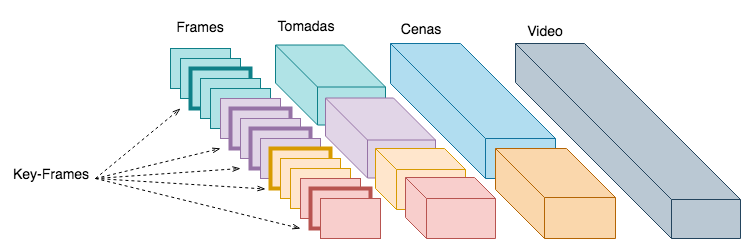
\includegraphics[width=\textwidth]{dados/figuras/video_structure.png}
       \fonte{Autoria própria.}
      \label{fig:video_sctructure}
    \end{figure}   

       Um conceito importante também relacionado ao vídeo é o quadro chave (do inglês \emph{key-frame}), ou quadro de cena. \citeonline{7848130} descrevem um quadro de cena como a imagem que define os pontos de início e fim de qualquer transição suave de imagens (o quadro que melhor representa a cena no geral). Quadros de cena são amplamente utilizados na produção de animações, em que normalmente o objeto ou sujeito da imagem se move em relação ao fundo \textit{(background)}. De acordo com \citeonline{mao2015sceneframe}, o quadro de cena deve possuir todos os elementos (pessoas, objetos, animais, etc.) exibidos na cena e o background deve ser altamente similar ao restante dos quadros. Na Figura \ref{fig:quadro_cena}, qualquer um dos cinco quadros pode ser eleito como o quadro de cena, pois todos têm os mesmos elementos (a mesma pessoa e o mesmo cachorro), além do \textit{background} ser praticamente o mesmo em todos os quadros.

 \begin{figure}[!htb]
      \centering
      \caption{Sequência com cinco quadros representando uma cena, retirado de um dos vídeos disponibilizados por \cite{reddy2013recognizing}.}
       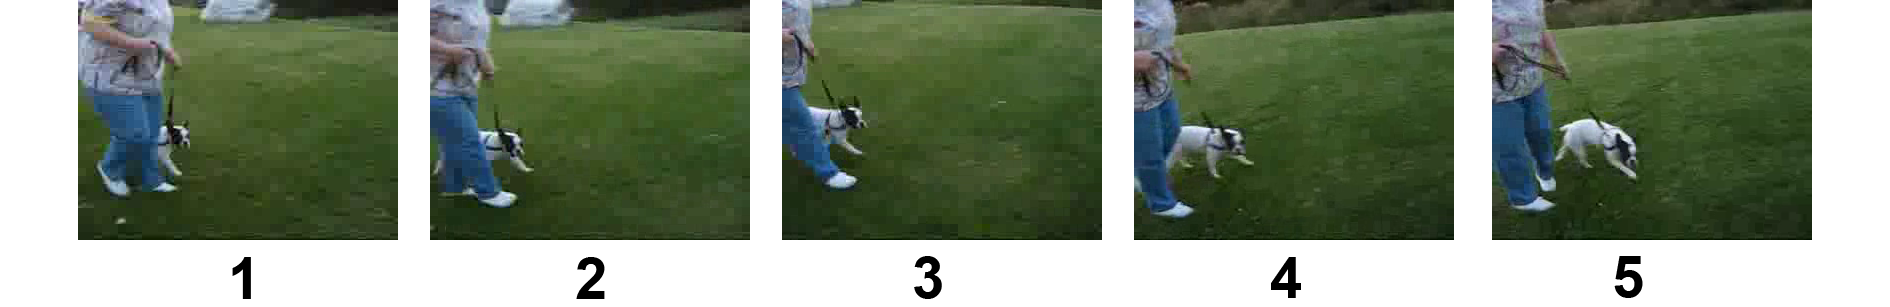
\includegraphics[width=0.96\textwidth]{dados/figuras/keyframe.png}
       \fonte{Autoria própria.}
      \label{fig:quadro_cena}
    \end{figure}   
    

    
    Em um vídeo existe também a dimensão espacial e a dimensão temporal. A dimensão espacial é classificada como a distribuição e a maneira com que os elementos estão organizados em um quadro. A dimensão temporal é a relação na qual os elementos e os quadros mudam ao longo de um vídeo \cite{hampapur2001comparison}.
    
% \section{Transformada de Haar}
% BOGDAN ------------------------ A explicação nesta seção está superficial demais, não tem referência, e a legenda da figura não explica direito o que cada sub-figura representa. Como assim "1/4 dos dados originais"? Como os detalhes são removidos? É simplesmente uma versão redimensionada da imagem no nível anterior? Se sim, isto é feito com interpolação ou sub-amostragem? Como são calculadas as derivadas? Mais importante que tudo: o que exatamente a transformada de Haar faz? Para que serve? De duas uma: ou vocês precisam detalhar muito melhor esta seção, incluindo a matemática da coisa; ou vocês removem esta seção, colocando uma referência e destacando o que é e para que serve a transformada de Haar quando ela for usada.

% Um conceito importante para dois dos algoritmos que serão apresentados (Sub Seções  \ref{wavelets} e \ref{sec:gradientes}) é o da transformada bidimensional de Haar. Ela faz parte da família de Transformadas de Wavelets, que são ferramentas matemáticas para decompor funções de forma hierárquica \cite{stollnitz1995wavelets}. No caso desta monografia essas funções são imagens. % que consiste na separação de um sinal (ou quadro, neste caso) em quatro partes: 

% Ao passar uma imagem pela Transformada de Haar 2D, 4 elementos são retornados: LL, LH, HL e HH. LL é a imagem original aplicada a um filtro passa-baixa e reduzida em metade do seu tamanho por um processo de interpolação. LH, HL,   

% \begin{enumerate}
% \item $LL$, que contém $1/4$ dos dados originais, removendo os detalhes;
% \item $LH$, que contém as derivadas na horizontal do quadro;
% \item $HL$, que contém as derivadas na vertical do quadro;
% \item $HH$, que contém as derivadas na diagonal do quadro.
% \end{enumerate}

% A transformada pode ser aplicada de forma recursiva, usando o quadro $I$ como entrada inicial do algoritmo e o $LL$ como entrada das chamadas subsequentes. Um exemplo do resultado da transformada de Haar pode ser visto na Figura \ref{fig:transf_haar}.

% BOGDAN ------------------------ Além de faltar uma explicação mais clara, a transformada de Haar não produz resultados negativos? Vocês devem remapear a imagem para apresentar (mapeando 0 como 0.5 ou 127).

%  \begin{figure}[h]
%       \centering
%       \caption{Sequência de recursões da transformada em uma imagem.}
%       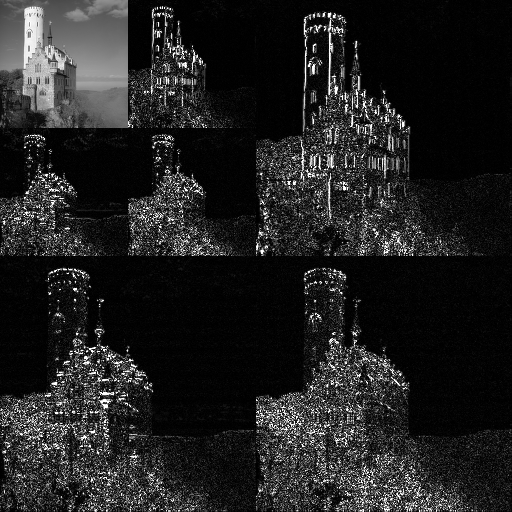
\includegraphics[width=0.96\textwidth]{dados/figuras/haar.png}      
%       \fonte{Autoria própria.}
%       \label{fig:transf_haar}
%     \end{figure}  

\section{Técnicas de detecção de cópias de vídeo}
    A detecção de cópias baseada em conteúdo (CBCD, do inglês \textit{Content Based Copy Detection}) é uma técnica para identificar vídeos através da criação de uma assinatura digital baseada em seu conteúdo \cite{jiang2011pku}. Apesar de o método ser utilizado em diversas aplicações, a detecção de cópias torna-se um desafio, considerando que a cópia pode sofrer ataques, distorções e transformações que dificultem a identificação do vídeo por um sistema automatizado.


\section{Tipos de ataques em vídeos}
\label{sec:ataques}

	Para evitar a detecção de duplicatas é comum a realização de ataques, ou distorções, nos vídeos. Existem várias maneiras de modificar um vídeo, como redimensionamento do tamanho, inserção ou remoção de alguns quadros, e alteração de cada quadro individualmente através da adição ou remoção de elementos, tais como bordas e legendas.

	No escopo deste trabalho são estudados 14 tipos de ataques para simular as táticas mais comuns utilizadas pelos apropriadores de conteúdo que tentam dificultar o reconhecimento de duplicatas. Os ataques são: adição de texto e legendas no vídeo, adição de marca d'água, adição de quadro ou bordas, redimensionamento da altura e largura dos quadros, eliminação de uma faixa ou região dos quadros, inversão/espelhamento, rotação, borramento, inversão de cores, alteração do formato de compressão dos quadros do vídeo, aceleramento do vídeo e, finalmente, remoção de quadros. A Figura \ref{fig:ataques} ilustra o resultado da aplicação de 8 dos ataques descritos acima em uma imagem.

    \begin{figure}[h]
        \centering
         \caption{Exemplos de ataques em uma imagem.}
        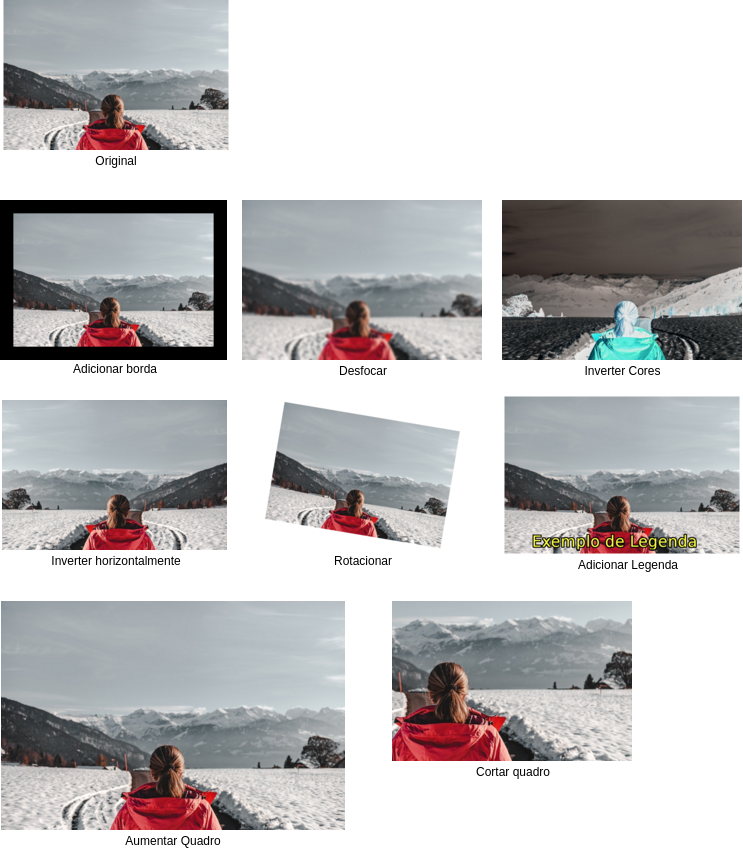
\includegraphics[width=0.8\textwidth]{dados/figuras/Ataques.png}
        \fonte{Autoria própria.}
       
        
    	\label{fig:ataques}
    \end{figure}

Os ataques dos tipos remoção de quadros, alteração do formato de compressão e aceleramento do vídeo só são perceptíveis quando visualizados em um dispositivo de exibição, como um computador, e por isso não estão representados na Figura~\ref{fig:ataques}. O ataque do tipo remoção de quadros consiste em remover alguns quadros ao longo do vídeo, e muitas vezes passa despercebido ao olho humano. O maior indicativo de que um vídeo sofreu esse ataque é observar a diferença temporal entre uma duplicata e o vídeo original, sendo que a duplicata terá uma duração menor em relação ao original. O ataque do tipo alteração da taxa de quadros também é realizado através da remoção de alguns quadros do vídeo, entretanto, o vídeo permanece com a mesma duração, pois os quadros restantes são na verdade exibidos por mais tempo\begin{comment}, ou seja, um quadro que era exibido durante um segundo passa a ser exibido durante dois segundos\end{comment}. O ataque do tipo alteração do formato de compressão é ainda mais difícil de ser percebido por humanos pois em muitos casos a diferença na imagem é muito sutil e geralmente ocorre em regiões que não são o foco da atenção do observador. Uma forma de descobrir se um vídeo sofreu esse tipo de ataque é observar o tamanho em disco da duplicata em relação do vídeo original, sendo que a duplicata normalmente ocupa menos espaço em disco devido à compressão com perda de dados do formato JPEG. A compressão JPEG é normalmente utilizada para compressão de imagens, mas foi usada nesta monografia por causar um efeito semelhante à compressão de vídeo.

% BOGDAN --------------- Este exemplo ficou bizarro, porque um quadro normalmente é exibido por 1/30 ou 1/60 segundo. =P (SOBRE ...ou seja, um quadro que era exibido durante um segundo passa a ser exibido durante dois segundos)

% BOGDAN --------------- Primeiro: JPEG é compressão COM perda. Segundo: JPEG normalmente não é usado para vídeos (formatos usados para vídeos normalmente exploram redundância temporal, coisa que o JPEG não tem).

Os ataques podem ainda ser classificados como geométricos, fotométricos ou temporais. Ataques geométricos afetam as características globais dos vídeos, ataques fotométricos afetam as características locais e, os ataques temporais, a dimensão temporal dos vídeos. A classificação dos ataques que serão utilizados nos vídeos deste trabalho é exibida na Tabela \ref{tab-classificacao-ataques}.

\begin{table}[!ht]
\centering
\caption{Classificação de ataques em vídeo.}
\label{tab-classificacao-ataques}
\begin{tabular}{|l|l|l|}
\hline
\# & \textbf{Ataque}                    & \textbf{Tipo} \\ \hline
1           & Aceleramento                       & Temporal      \\ \hline
2           & Adição de bordas                   & Fotométrico   \\ \hline
3           & Adição de texto (legendas)         & Fotométrico   \\ \hline
4           & Alteração do formato de compressão & Fotométrico   \\ \hline
5           & Borramento                         & Fotométrico   \\ \hline
6           & Eliminação de faixa ou região      & Geométrico    \\ \hline
7           & Espelhamento                       & Geométrico   \\ \hline
8           & Inversão de cores                  & Fotométrico   \\ \hline
9           & Marca d'água                       & Fotométrico   \\ \hline
10          & Redimensionamento                  & Geométrico    \\ \hline
11          & Remoção de quadros                 & Temporal      \\ \hline
12          & Rotação                            & Geométrico    \\ \hline
\end{tabular}
\end{table}





\section{Assinaturas de vídeo}
\label{sec:assinatura} 
    
	Uma assinatura de vídeo é definida como um vetor de características que representa um vídeo e o diferencia de outros \cite{lee2008robust}. Em outras palavras, a assinatura é uma representação de um vídeo em uma estrutura de dados. 
        
	Para um algoritmo de geração de assinatura ser considerado eficiente, é importante que três características sejam consideradas: robustez, singularidade e eficiência de busca. De acordo com \citeonline{lee2008robust}, uma assinatura é considerada robusta caso o descritor gerado para um vídeo modificado seja similar ao descritor do vídeo original. A singularidade, ou unicidade, é a capacidade do algoritmo gerar assinaturas diferentes para vídeos perceptivelmente diferentes. Por fim, eficiência de busca é a capacidade da assinatura  ser utilizada por uma aplicação para buscas em banco de dados de larga escala. Nesta monografia, são avaliadas apenas a robustez e a singularidade das assinaturas.   

    Existem duas classes principais de algoritmos para descrever vídeos e então gerar assinaturas, são elas: locais e globais. Cada classe tem características que a faz mais robusta para combater diferentes tipos de ataques, sendo então cada uma indicada para situações diferentes.
    
    Descritores locais geram assinaturas baseadas em pontos ou regiões de interesse de cada quadro do vídeo. Os pontos de interesse são determinados a partir de regiões que possuem uma acentuada variação na orientação do gradiente dos elementos presentes em um quadro, como, por exemplo, o enquadramento de uma porta ou o pico de uma montanha. As regiões de interesse são determinadas pelos \textit{pixels} ao redor de um ponto de interesse e ajudam a determinar os limites dessas regiões \cite{radhakrishnan2007content}. Esses descritores normalmente são robustos contra variações fotométricas (borrados, variação de luminância e cor, ruído e compressões) e podem ser custosos computacionalmente devido aos cálculos necessários para determinar os pontos de interesse \cite{naini2014vanishing}. Um descritor local consiste normalmente de três etapas: detecção das características, descrição das características e combinação das características \cite{chen2010zernike}.

    A classe de descritores globais, ao contrário dos descritores locais, geram assinaturas utilizando informações pertinentes ao quadro como um todo, como por exemplo a luminância total do quadro. Esses podem apresentar vantagens em relação aos descritores locais, pois normalmente é menos custoso em termos computacionais trabalhar com informações gerais do quadro do que realizar uma análise para determinar pontos de interesse. Além disso, os descritores globais podem gerar assinaturas mais robustas quando considerados os ataques geométricos às imagens \cite{law2007video}. 
    
%==================================================================================
\section{Algoritmos para geração de assinaturas}

% BOGDAN ----------- Quais são os tamanhos esperados para cada assinatura? Outra coisa: é bom indicar claramente se cada descritor é local ou global. Algumas das descrições estão bem vagas.
	
	A seguir é apresentado o estudo dos sete algoritmos que foram selecionados e implementados para a realização dos experimentos.


% --------------------------------------------------------------------------------------------------
%
% MEDIDA ORDINAL
%
% --------------------------------------------------------------------------------------------------
\subsection{Assinatura baseada na medida ordinal}
\label{sec:med_ordinal}

	O algoritmo proposto por \citeonline{hua2004robust} baseia-se na intensidade dos \textit{pixels} de cada quadro para compor a assinatura. Primeiramente, a taxa de amostragem, ou seja, a taxa de quadros por segundo (FPS) do vídeo de entrada é padronizada, para que a assinatura gerada fique mais compacta e seja tolerante a diferentes formatos de compressão. Além disso, o vídeo é convertido para escala de cinza.

	Após esse pré-processamento, cada quadro é particionado em $M \times N$ blocos, como pode ser observado na Figura~\ref{fig:medidaord}, e a intensidade média para cada um dos blocos é computada. O descritor é então formado pela concatenação dos vetores em cada bloco. O método é resumido na Figura~\ref{fig:dia_ordinal}. O tamanho final de uma assinatura baseada em medida ordinal é $N \times M \times k$ onde $k$ é o número de quadros de um vídeo. Para esta implementação, foi utilizado $M = 5$ e $N = 5$.

	\begin{figure}[!htb]
        \centering
        \caption{Exemplo de divisão em blocos, cálculo das intensidades médias e ordem atribuída a cada valor.}
        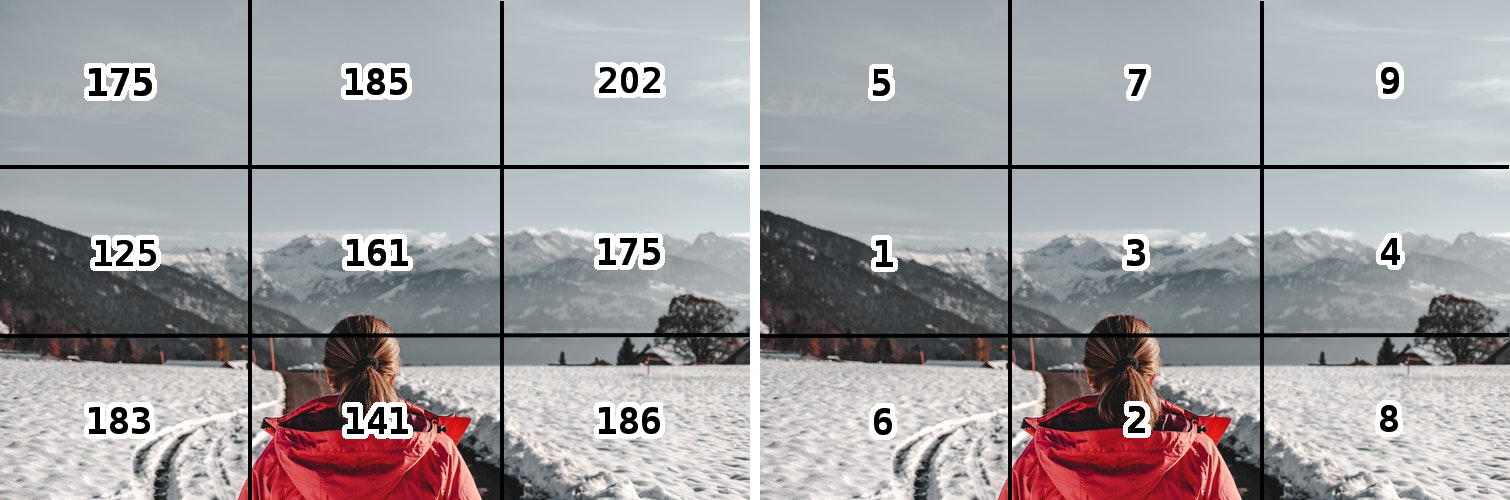
\includegraphics[width=0.8\textwidth]{dados/figuras/mo_final.png}
        \fonte{Autoria própria.}
        \label{fig:medidaord}
    \end{figure}

 \begin{figure}[!htb]
      \centering
      \caption{Diagrama do algoritmo baseado em medida ordinal.}
      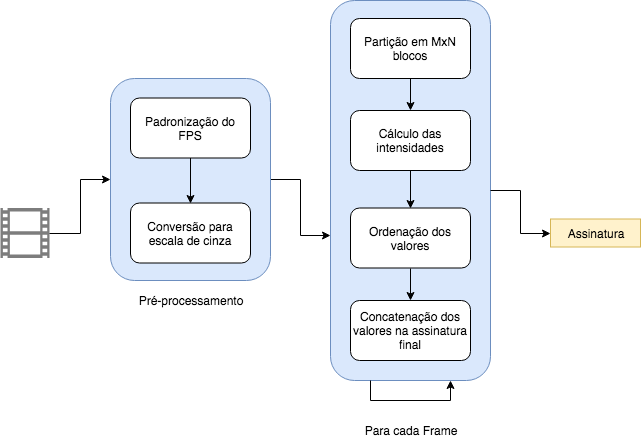
\includegraphics[width=0.96\textwidth]{dados/figuras/diagramas/Diag-MO}
      \fonte{Autoria própria.}
       	\label{fig:dia_ordinal}
    \end{figure}  

% --------------------------------------------------------------------------------------------------
%
% GRADIENTE
%
% --------------------------------------------------------------------------------------------------


\subsection{Assinatura baseada em gradientes}
\label{sec:gradientes}

	O algoritmo proposto por \citeonline{lee2008robust} utiliza a distribuição dos gradientes para geração de assinaturas. O primeiro passo é definir uma taxa de quadros por segundo (FPS) fixa, além da conversão para escala de cinza. Também é realizado o redimensionamento dos quadros, tornando o método robusto independente da mudança de resolução do vídeo. Em seguida, os gradientes $\mathbb{G}x$ e $\mathbb{G}y$ dos pixels de cada quadro são calculados como mostra a Equação \ref{eq:gmatrix}.

\begin{equation}
  \label{eq:gmatrix}
  \begin{bmatrix}
    \mathbb{G}x
    \\ 
    \mathbb{G}y
  \end{bmatrix}= 
  \begin{bmatrix}
    \partial I/\partial x
    \\ 
    \partial I/\partial y
  \end{bmatrix}=
  \begin{bmatrix}
    $I$(x+1, y) - $I$(x-1,y)
    \\ 
    $I$(x, y+1) - $I$(x,y-1)
  \end{bmatrix}
\end{equation}
    
	O quadro é então dividido em $M\times N$ blocos, para os quais é determinado o valor do centroide dos gradientes, criando assim um vetor com $M \times N$ elementos. Para isso, são computadas as imagens de magnitude \textit{$w(x,y)$} e a orientação \textit{$\Theta(x,y)$}, conforme mostra a Equação \ref{eq:mag-or}.
    
\begin{equation}
	\label{eq:mag-or}
    w(x,y) = \sqrt{\mathbb{G}x^{2} + \mathbb{G}y^{2}}
\qquad
\Theta(x,y) = tan^{-1}\left (\frac{\mathbb{G}y}{\mathbb{G}x} \right)
\end{equation}
    
    Em seguida o centroide para cada bloco $b[i]$ é obtido a partir do somatório do produto da magnitude e orientação, dividido pela somatória de todas as magnitudes daquele bloco, como pode ser observado na Equação \ref{eq:gradientes}.
    
% BOGDAN ----------------------- Sério que a conta é esta?? Eu fui até ver o artigo original para conferir, porque esta conta tem um problema: ela não leva em conta a natureza cíclica das orientações. Ou seja, uma média entre 359 graus e 1 grau dá... 180 graus, que é um contraste no sentido oposto!
    
\begin{equation}
	\label{eq:gradientes}
	b[i] = \frac{\sum_{x,y \in b[i]} w(x,y)\Theta (x,y)}{\sum_{x,y \in b[i]} w(x,y)}
\end{equation}

A assinatura final é obtida pela concatenação desses vetores (Figura \ref{fig:dia_gradiente}). O tamanho final de uma assinatura baseada em gradiente é $N \times M \times k$ onde $k$ é o número de quadros de um vídeo. Para esta implementação, foi utilizado $M = 3$ e $N = 4$.  

 \begin{figure}[h]
      \centering
      \caption{Diagrama do algoritmo baseado em gradientes.}
      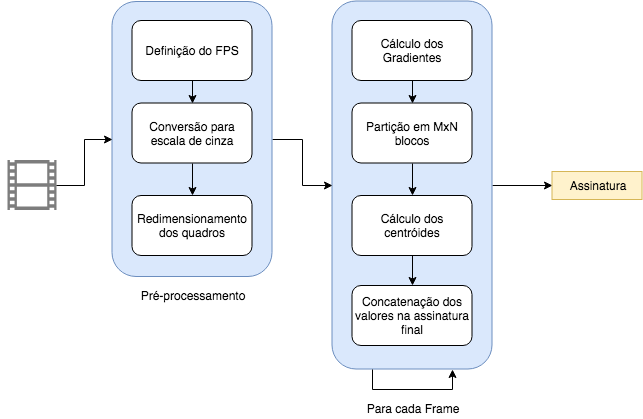
\includegraphics[width=0.96\textwidth]{dados/figuras/diagramas/Diag-Gradiente}
      \fonte{Autoria própria.}
       	\label{fig:dia_gradiente}
    \end{figure}  
    
% --------------------------------------------------------------------------------------------------
%
% FRAME DIFF
%
% --------------------------------------------------------------------------------------------------

\subsection{Assinatura baseada na diferença entre quadros}
\label{sec:framediff}

  O algoritmo proposto por \citeonline{cook2011efficient} utiliza características globais de luminância e de diferença de luminância intra-quadros. Para cada quadro do vídeo são coletadas características primárias, como a luminância total ($Y$), obtida através da soma da luminância de todos os pixels do quadro; a luminância máxima ($Y_{max}$), que é o valor do pixel mais brilhante do quadro; e a luminância diferencial ($dY$), que é a diferença absoluta de luminância pixel a pixel do quadro atual com o quadro que estava visível a 100 milissegundos, a diferença resultante é somada conforme mostra a Equação \ref{eq:framediff}. Os valores obtidos são então normalizados, levando em conta a dimensão dos quadros do vídeo.
  
\begin{equation}
	\label{eq:framediff}
	dY = \sum_{x,y \in  I,J} |I(x,y) - J(x,y)|
\end{equation} 

   Após a obtenção das características primárias, um filtro passa-baixa Gaussiano é utilizado para suavizar a assinatura, como pode ser observado na Figura \ref{fig:framediff-passa-baixa}. A assinatura é a concatenação dos somatórios das diferenças entre quadros e a luminância total de cada quadro. O tamanho final de uma assinatura baseada em diferença entre quadros é $N \times M \times k$ onde $k$ é o número de quadros de um vídeo. Para esta implementação, foi utilizado $M = 5$ e $N = 5$.
   %Além disso, duas outras características, quietude e créditos, são derivadas das características principais e visam medir o quão imóvel uma sequência de quadros é. Para isso, são definidas as medidas "Quietude" (Equação \ref{eq:framediff-stillness}) e "Créditos" (Equação \ref{eq:framediff-credits}).

%   \begin{equation}
%     \label{eq:framediff-stillness}
%     Quietude = 100 \times \left(\sqrt{\frac{\ln\frac{dY}{A}}{\ln256}}\right) \\
%   \end{equation}

%   \begin{equation}
%     \label{eq:framediff-credits}
%     Créditos = 100 \times \frac{\frac{Y_{max}}{256} + \left( 1 - \left( \frac{\ln\frac{Y}{A}}{\ln256} \right)^2\right)}{2}
%   \end{equation}


\begin{figure}[h]
\centering
	\caption{Linha azul mostra os valores originais do vetor $dY$ e a linha alaranjada mostra os valores pós filtro passa-baixa.}
  	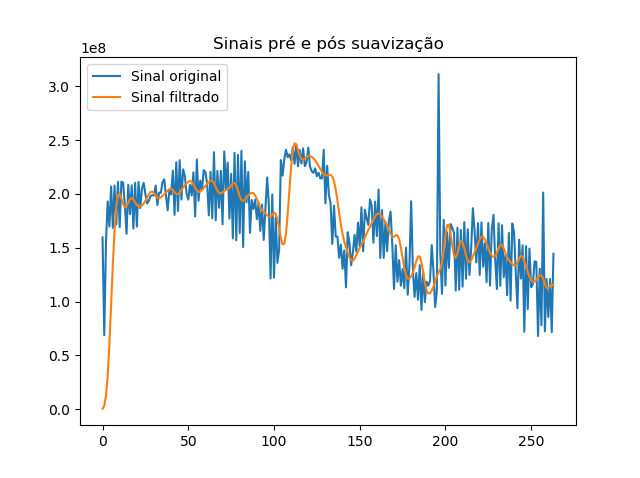
\includegraphics[width=0.7\textwidth]{dados/figuras/filtro_passa_baixa}
  	\fonte{Autoria própria.}
  \label{fig:framediff-passa-baixa}
\end{figure}

% A Figura \ref{fig:framediff-comparacao} mostra a característica $dY$ plotada para um vídeo original e sua versão distorcida com efeitos de borramento e adição de legenda, além de mostrar os valores de $dY$ para outro vídeo não relacionado.

 \begin{figure}[h]
      \centering
      \caption{Diagrama do algoritmo baseado na diferença entre quadros.}
      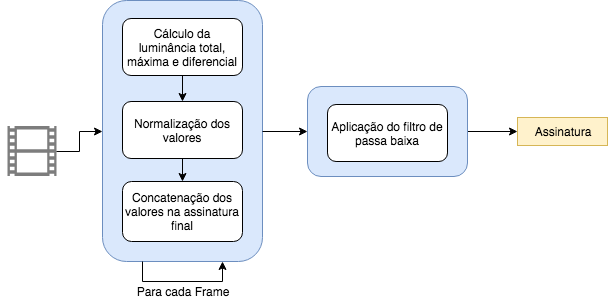
\includegraphics[width=0.96\textwidth]{dados/figuras/diagramas/Diag-FrameDiff}
      \fonte{Autoria própria.}
       	\label{fig:dia_framediff}
    \end{figure}  

%% --------------
%% TODO: explicar comparação
%% --------------

%   Dados dois quadros $\mathbb{I}$ e $\mathbb{J}$, a assinatura temporal desenvolvida por \cite{cook2011efficient} utiliza dois componentes principais para sua construção. O primeiro é a luminância total $Y$, ou seja, a soma dos \textit{pixels} do \textit{frame}, representando o brilho total da imagem. O outro parâmetro é $dY$, ou diferencial de luminância, sendo a diferença do quadro atual com o quadro anterior. $dY$ é uma métrica para saber o quanto a luminância varia com a mudança dos quadros no vídeo.  Essa variação pode acontecer, segundo o autor, a partir do movimento da câmera, corte entre cenas e objetos e pessoas que entram ou saem de cena. 
    
%    O  valor de $dY$ pode ser obtido através da Equação \ref{eq:framediff} \cite{sylvio2015}: 

% Portanto cada \textit{frame} será representando por uma tupla $(Y, dY)$.

 

% --------------------------------------------------------------------------------------------------
%
% SCENE FRAME
%
% --------------------------------------------------------------------------------------------------

\subsection{Assinatura baseada em quadros de cena}

  A abordagem proposta por \citeonline{mao2015sceneframe} é baseada na assinatura de quadros de cena (Seção \ref{sec:video}). De acordo com os autores, os quadros de cena podem ser \textit{intraframes}, ou seja, quadros que iniciam tomadas, quanto \textit{interframes}, contanto que sigam as características descritas na Seção \ref{sec:video}, ou seja, possuir todos os mesmos elementos dos quadros restantes e o mesmo \textit{background}.

A assinatura individual de cada quadro é calculada conforme os passos descritos na Figura \ref{fig:dia_sceneframe}. Os quadros passam por um pré-processamento, onde o componente de luminância pertencente ao espaço HSL (\textit{hue, saturation, lightness}) da imagem é extraído, uma vez que apenas este valor é considerado pelo algoritmo. O quadro é recortado mantendo-se apenas sua região central e redimensionado para o tamanho definido de $108\times132$ pixels. Além disso, é aplicado o filtro passa-baixa Gaussiano.

\begin{figure}[h]
  \centering
  \caption{Diagrama do algoritmo baseado em quadros de cena.}
  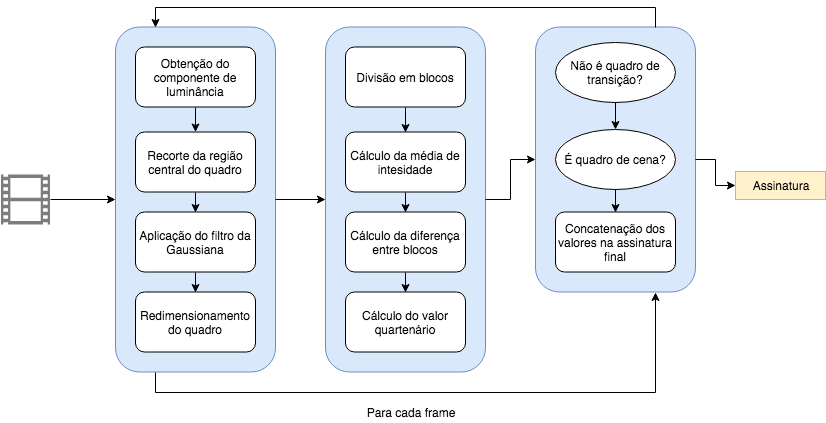
\includegraphics[width=\textwidth]{dados/figuras/diagramas/Diag-SceneFrame}
  \fonte{Autoria própria.}
  \label{fig:dia_sceneframe}
\end{figure}

Após o processamento inicial, o quadro é então dividido em $144$ pedaços menores, de tamanho $9\times11$ pixels, cuja intensidade média irá compor parte da assinatura deste quadro. Além dos $144$ valores, o descritor é composto também por $576$ elementos diferenciais, totalizando $720$ valores. Para obter esses elementos diferenciais, cada fragmento é dividido em oito elementos menores, conforme a Figura \ref{fig:divsceneframe}, e então é realizada a subtração de $a - b$, $c - d$, $e - f$ e $g - h$.

\begin{figure}[h]
  \centering
    \caption{Divisão da imagem para cálculo dos elementos diferenciais.} 
    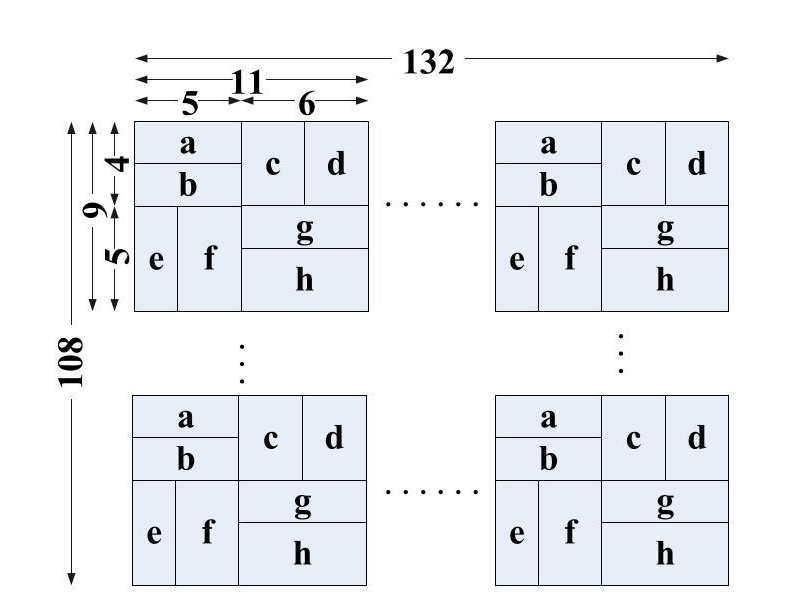
\includegraphics[width=\textwidth]{dados/figuras/sf_division.png}
    \fonte{\cite{mao2015sceneframe}.}
    \label{fig:divsceneframe}
\end{figure}

O artigo também propõe uma alternativa para diminuir o espaço de memória utilizado para armazenar as assinaturas, visto que o banco de dados dos vídeos pode ser grande. Para isso, é proposta uma técnica chamada quantificação quaternária, na qual os valores são classificados de acordo com um limiar, calculado dinamicamente para cada quadro. O primeiro limiar, utilizado para as $144$ médias de intensidade, é obtido da seguinte maneira: considere que $m_i$ representa cada valor dentro do conjunto $M$ de médias de intensidade. Para todo $m_i$ em $M$, é calculado o valor absoluto $a_i = \lvert m_i - 128 \rvert$, obtendo novos valores $A$. Os valores de $A$ são, então, organizados em ordem crescente. Para separar os valores em 4 faixas, é utilizado o triségimo-sexto valor do conjunto ordenado A, definindo o limiar ThM. O limiar $ThM$ utilizado será $a_i$ onde $i = \lfloor 0.25*144 \rfloor$. Finalmente, cada valor $m_i$ é então definido através da Equação \ref{eq:mediaquart}.

\begin{equation}
	\label{eq:mediaquart}
	m_i = 
     \begin{cases}
       \text{3,} &\quad\text{Se } m_i-128 > \text{ThM} \\
       \text{2,} &\quad\text{Se } 0 < m_i - 128 \le \text{ThM} \\
       \text{1,} &\quad\text{Se } -\text{ThM} < m_i - 128 \le 0 \\
       \text{0,} &\quad\text{Se } m_i - 128 \le -\text{ThM} \\ 
     \end{cases}
\end{equation}

A mesma lógica é aplicada para os $576$ valores diferenciais, porém, para estes não é necessário realizar as subtrações por $128$.

Com os valores quaternizados, a assinatura será adicionada ao vetor final de resultado com duas condições: o quadro não pode ser um quadro de transição, chamado de \textit{black frame} pelos autores, e deve ser considerado quadro de cena. Portanto, a assinatura final é composta de valores no intervalo de $\left[0,3\right]$.

% --------------------------------------------------------------------------------------------------
%
% RBP
\subsection{Assinatura baseada em padrões binários por região}
% --------------------------------------------------------------------------------------------------


O descritor apresentado por \citeonline{kim2014rotation} propõe criar uma assinatura que seja robusta para ataques de rotação e espelhamento. Trata-se de um descritor local que utiliza a dimensão espacial dos quadros do vídeo para a extração da assinatura. 

% BOGDAN ------------ Como são estes padrões??? (SOBRE Dessas sub-regiões, o algoritmo gera dois padrões binários com...)

O método divide o quadro em regiões circulares, e então divide os círculos em sub-regiões, ou seja, sub-círculos, como pode ser observado na Figura \ref{fig:aneis_rbp}. Dessas sub-regiões, o algoritmo gera dois padrões binários com a justificativa de preservar as informações da dimensão espacial do quadro e dessa forma manter a robustez da assinatura em relação aos ataques de rotação e espelhamento. O  primeiro padrão binário  \textit{(RBP, Region Binary Pattern)} representa uma única região circular, enquanto o segundo padrão binário representa a relação entre a primeira região e as regiões adjacentes. Após, esses dois padrões são agrupados e concatenados em um vetor, que é a assinatura resultante do algoritmo. A Figura \ref{fig:dia_rbp} ilustra o fluxo geral do algoritmo.

 \begin{figure}[h]
      \centering
      \caption{Divisão de um quadro em regiões circulares.}
      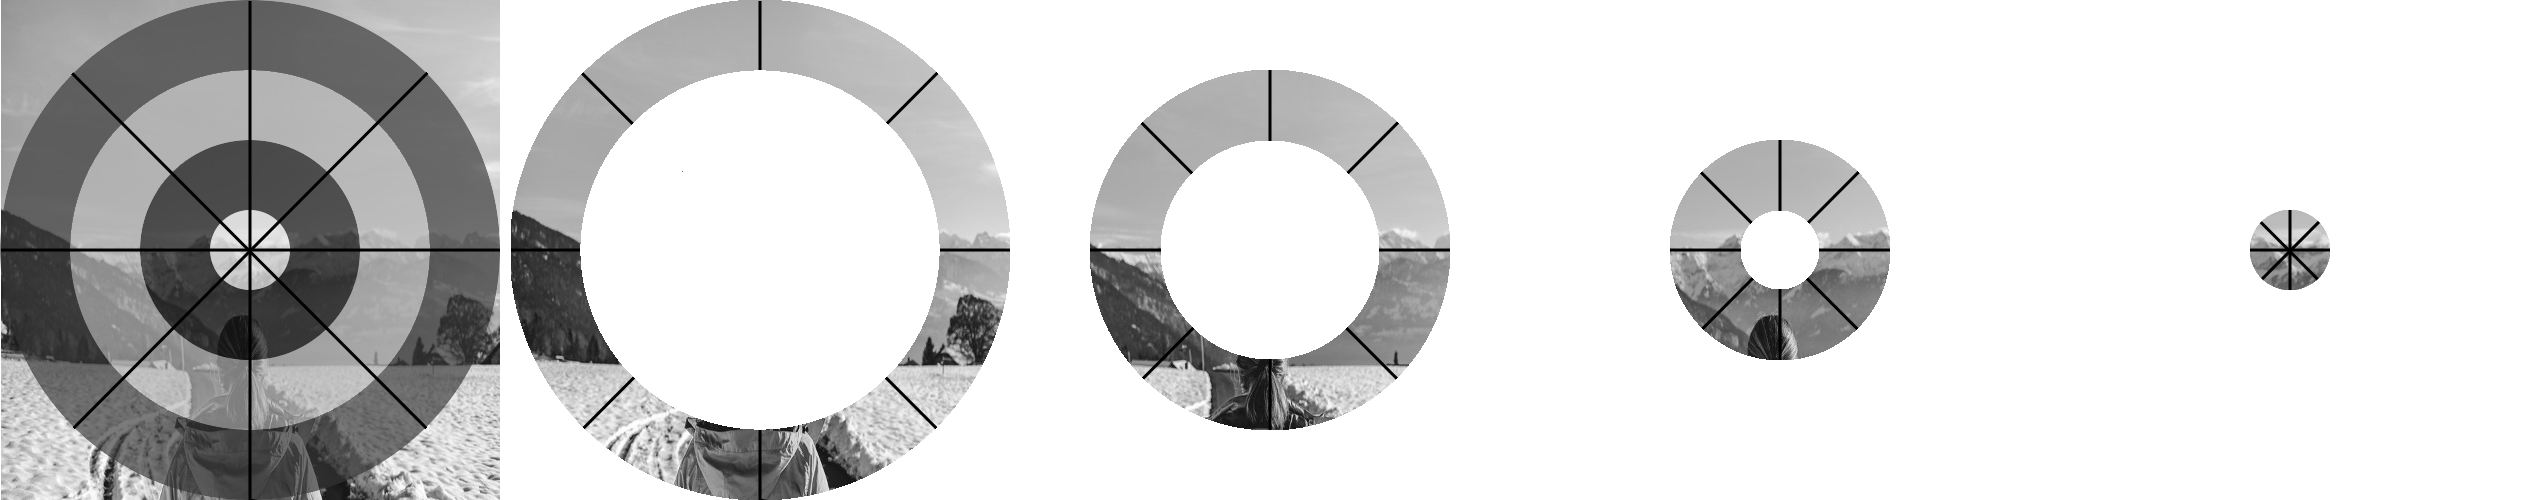
\includegraphics[width=0.96\textwidth]{dados/figuras/brp_aneis}
      \fonte{Autoria própria.}
       	\label{fig:aneis_rbp}
    \end{figure} 

 \begin{figure}[h]
      \centering
      \caption{Diagrama do algoritmo baseado padrões binários por região.}
      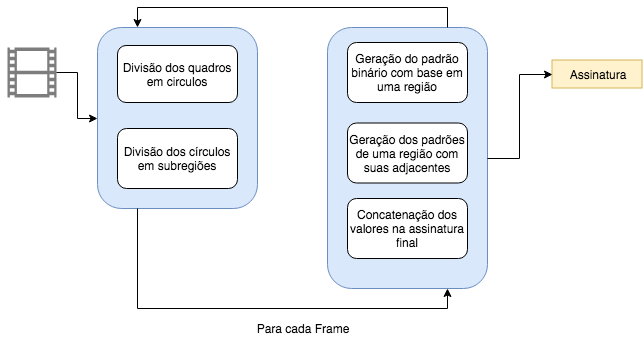
\includegraphics[width=0.96\textwidth]{dados/figuras/diagramas/Diag-RBP}
      \fonte{Autoria própria.}
       	\label{fig:dia_rbp}
    \end{figure}  

    
% --------------------------------------------------------------------------------------------------
%
% WAVELETS
%
% --------------------------------------------------------------------------------------------------

\subsection{Assinatura baseada em wavelets}
\label{wavelets}

Esta abordagem foi escolhida por ter sido projetada especialmente para ser robusta a uma variedade de ataques fotométricos, como modificações em contraste, brilho, contaminação por ruído e desfoque, inserção de logos, bordas e mudança de formato do quadro. Para a abordagem se tornar ainda mais robusta a esses ataques, \citeonline{Dutta2013} também realizam uma etapa de pré-processamento em que possíveis bordas dos quadros são removidas, então o ruído das imagens é removido através de um filtro gaussiano e finalmente o histograma de cada quadro é equalizado. 

Após a etapa de pré-processamento, para serem utilizados como entrada para este algoritmo, os vídeos devem ser transformados para escala de cinza e ter suas intensidades normalizadas para o intervalo $[0,1]$. A assinatura proposta por \citeonline{Dutta2013} é composta de uma parte baseada na transformada de Haar bidimensional e em outra parte baseada na distribuição espacial de gradientes. A transformada de Haar faz parte da família de Transformadas de Wavelets, que são ferramentas matemáticas para decompor funções de forma hierárquica \cite{stollnitz1995wavelets}. No caso desta monografia essas funções são imagens. 

% Um conceito importante para dois dos algoritmos que serão apresentados (Sub Seções  \ref{wavelets} e \ref{sec:gradientes}) é o da transformada bidimensional de Haar. Ela faz parte da família de Transformadas de Wavelets, que são ferramentas matemáticas para decompor funções de forma hierárquica \cite{stollnitz1995wavelets}. No caso desta monografia essas funções são imagens. % que consiste na separação de um sinal (ou quadro, neste caso) em quatro partes: 

% Ao passar uma imagem pela Transformada de Haar 2D, 4 elementos são retornados: LL, LH, HL e HH. LL é a imagem original aplicada a um filtro passa-baixa e reduzida em metade do seu tamanho por um processo de interpolação. LH, HL,   

% \begin{enumerate}
% \item $LL$, que contém $1/4$ dos dados originais, removendo os detalhes;
% \item $LH$, que contém as derivadas na horizontal do quadro;
% \item $HL$, que contém as derivadas na vertical do quadro;
% \item $HH$, que contém as derivadas na diagonal do quadro.
% \end{enumerate}


 Para gerar a assinatura são aplicadas $n$ iterações da transformada de Haar sobre a imagem de entrada $I$, para computar as bandas $HH, LH, HL$ e $LL$.  Então são computadas as energias das bandas $LH$, $HL$, $HH$, conforme a Equação \ref{eq:bandasH}.
 
 \begin{equation}
	\label{eq:bandasH}
	\frac{1}{MN}\sum_{x=1}^M \sum_{y=1}^N |I(x,y)|
\end{equation} 
 
 
 
 %Para i de 1 até $n$, onde $n$ é o número de iterações da transformada de Haar:
%   \begin{enumerate}
%     \item Aplicar a transformada de Haar sobre $I$ para obter um vetor com ($LL, LH, HL, HH$);
%     \item Computar energia de $LH$, $HL$, $HH$ \footnote{$  \frac{1}{MN}\sum_{x=1}^M \sum_{y=1}^N |\mathbb{I}(x,y)|$};
%   \end{enumerate}

 Em seguida, computa-se somente a energia do último valor de $LL$ da subimagem $I$. Finalmente, os valores de energia obtidos nos passos anteriores são concatenados em um vetor, resultando na assinatura do vídeo.

% \begin{figure}[h]
%   \centering
%   \begin{tabular}{ccc}
%     \centering
%     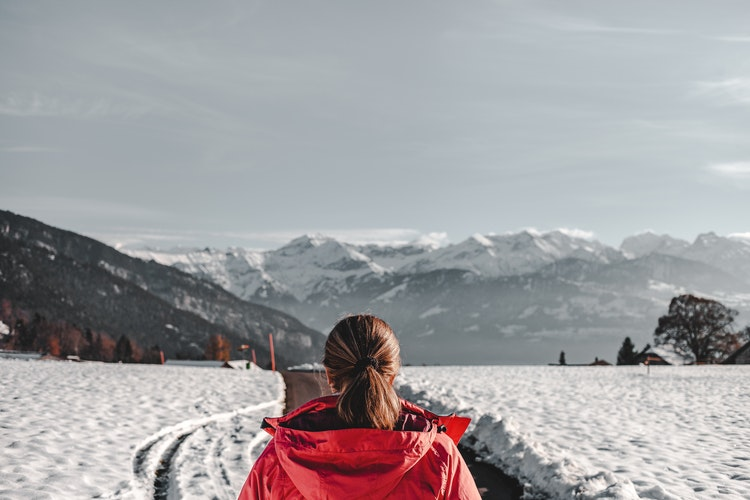
\includegraphics[width=0.45\textwidth]{dados/figuras/original} & 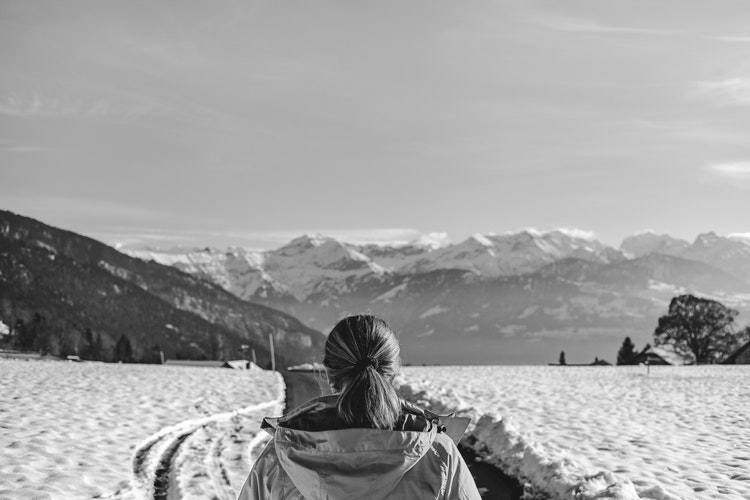
\includegraphics[width=0.45\textwidth]{dados/figuras/original_bw} \\ 
%      a. Quadro original & b. Quadro em escala de cinza \\
%     \multicolumn{2}{c}{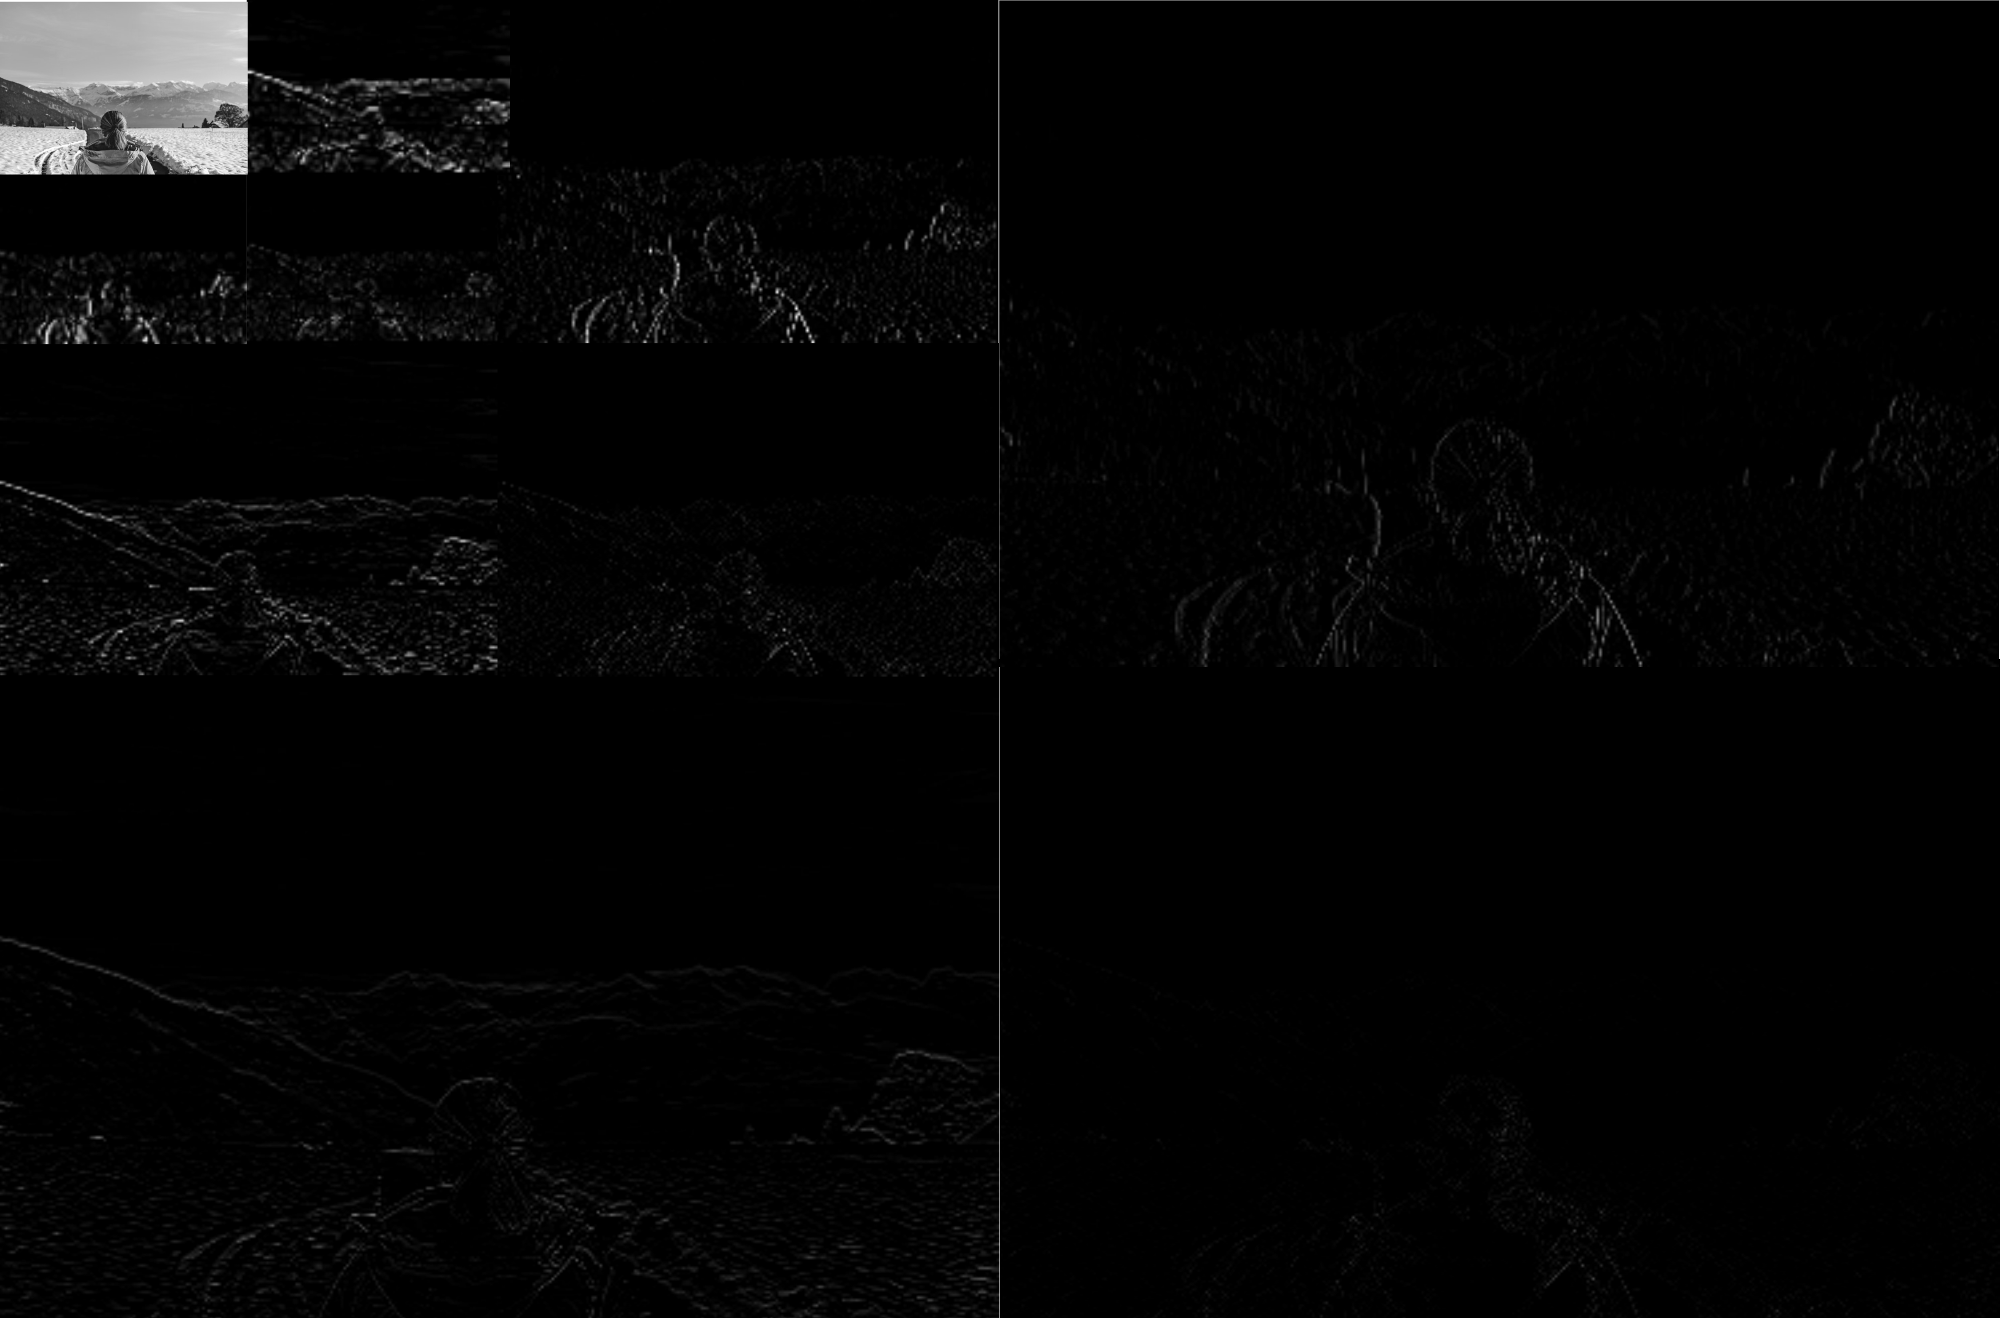
\includegraphics[width=0.94\textwidth]{dados/figuras/wavelet_result_menor}} \\
%     \multicolumn{2}{c}{c. Após transformada de Haar}
%   \end{tabular}
%   \caption{Sequência de transformações feitas pelo algoritmo}
% %   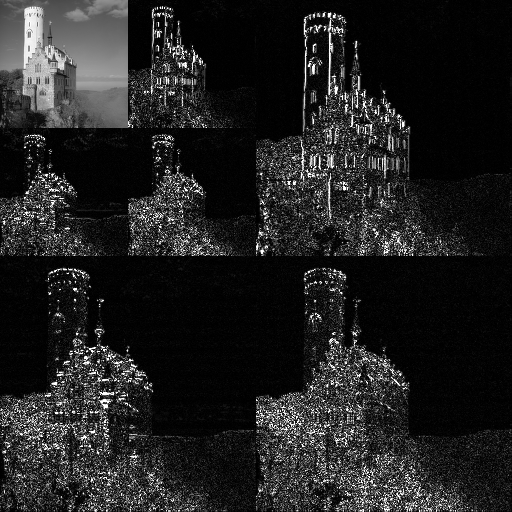
\includegraphics[width=0.8\textwidth]{dados/figuras/haar.png}
% %   \caption{Resultado da Transformada de Haar. Os cantos superior direito, inferior esquerdo e inferior direito são, respectivamente, a derivada na horizontal(LH),derivada na vertical(HL) e derivada na diagonal(HH). O canto superior esquerdo é subdividido $N$ vezes em LH,HL e HH até o último nível em que não há mais divisão e que se chama LL}
%   \label{figure:haar}
% \end{figure}



% A assinatura é gerada a partir de um quadro $I$ já pré-processado, em que é aplicada a transformada de Haar com um nível e obter um vetor com $LL,LH,HL,HH$. Então, computa-se o gradiente de $LL$ \footnote{A imagem LL é usada pois contém menos ruído que a imagem original graças à transformada de Haar} e a imagem de gradiente é dividida em $N_p$ partições com o mesmo tamanho. O penúltimo passo é, para cada partição, computar um histograma de gradiente. Finalmente, os histogramas são concatenados para obter o a assinatura.


 \begin{figure}[h]
      \centering
      \caption{Diagrama do algoritmo baseado em wavelets.}
      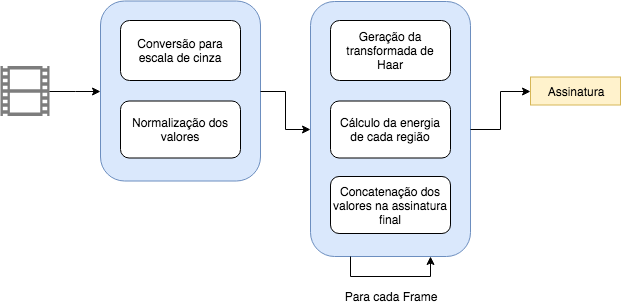
\includegraphics[width=0.96\textwidth]{dados/figuras/diagramas/Diag-Wavelets}
      \fonte{Autoria própria.}
       	\label{fig:dia_wavelet}
    \end{figure}  
    
% --------------------------------------------------------------------------------------------------
%
% CAMERA MOTION
%
% --------------------------------------------------------------------------------------------------

\subsection{Assinatura baseada no movimento da câmera}
\label{wavelets}


% BOGDAN --------------- Existem vários algoritmos de fluxo ótico. Qual é usado aqui?


%detec'ão de movimento
%capaz de identificar movimento de camera em 95% dos testes e detectar objetos de "background e foreground"
%dois passos: 1. determinar uma regiao de fluxo óptico no video; 2. estimar o movimento da camera na regiao de fluxo óptico
%o fluxo óptico de uma imagem I para uma posterior imagem J é uma função F que para o domínio da imagem D, associa um vetor de velocidade F(u) tal que u + F(u) pertencem ao domínio D.
%este algoritmo assume que o fluxo óptico f está fixado em um conjunto de pontos, que formam uma lista de vetores. o algoritmo requer que cada vetor f(i) tenha um peso correspondente (wi), que representa a sua confiabilidade.



O algoritmo proposto por \citeonline{minetto2007reliable} detecta o movimento da câmera em um vídeo em três níveis: \textit{pan} (movimentos para esquerda ou direita, sem mover a base da câmera), \textit{tilt} (movimentos para cima ou para baixo, sem mover a base da câmera), \textit{zoom} (movimentos de aproximação ou de afastamento) e roll (movimento de rotação com câmera voltada para o mesmo ponto). O algoritmo é capaz de determinar o movimento da câmera em 95\% das tomadas nos casos de testes realizados pelos autores, em um ambiente onde 98\% das tomadas haviam algum tipo de movimento de câmera. A Figura~\ref{fig:example_cameramotion} apresenta um exemplo de movimentação de câmera entre dois quadros.

\begin{figure}[h]
	\centering
	\caption{Movimento da câmera entre dois quadros consecutivos. Os pontos as direita representam os vetores de movimento. Neste caso há uma combinação de \textit{pan} para a esquerda e \textit{tilt} para cima.}
	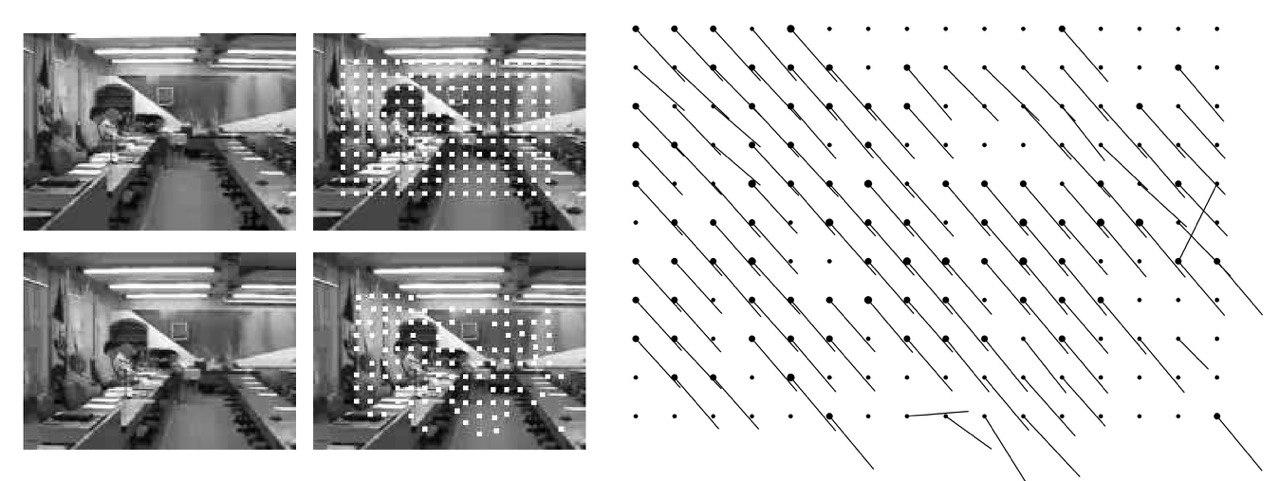
\includegraphics[width=\textwidth]{dados/figuras/cameramotion-example}
	\fonte{\cite{minetto2007reliable}}
	\label{fig:example_cameramotion}
\end{figure}

Seu funcionamento, segundo \citeonline{minetto2007reliable} é dividido em duas etapas. A primeira é determinar uma região de fluxo óptico, ou seja, uma região no vídeo onde os movimentos de câmera serão monitorados. A segunda etapa é estimar os movimentos da câmera dentro dessa região de fluxo óptico.

O fluxo óptico de uma imagem $I$ para uma imagem subsequente $J$ é uma função $f$, que, para cada ponto $u$ do domínio $D$ da imagem, associa um vetor de velocidade $f(u)$, tal que $u + f(u)$ pertencem ao domínio $D$. O algoritmo assume que o fluxo está fixado em um conjunto de pontos na região de fluxo óptico e formam uma lista de vetores na qual cada vetor tem um peso correspondente, que representa a sua confiabilidade. 

% Diagrama: 1) Definição de uma grade de pontos sobre a imagem, 2) Cálculo de vetores de movimento e peso para cada ponto da grade com um algoritmo de rastreamento (KLT).


% Para cada ponto, existe um vetor de movimento e um peso que considera a textura local (para melhor rastreamento). Quanto mais fácil o rastreamento deste ponto, ou seja, quanto maior a diferença de textura, maior o peso.

% Os valores canônicos de movimento são então aproximados: pan, tilt e zoom (o que é cada um já explicado no texto).

% A variação dos movimentos é calculada com base em dois frames consecutivos e nos pesos atribuídos aos vetores. Os pontos entre duas imagens são relacionados atraves de uma modificação do algoritmo de Kanade-Lucas-Tomasi, que considera também os pesos calculados no primeiro passo. 

% Objetos em movimento podem comprometer o cálculo do fluxo ótico, por isso é realizado um ajuste de pesos. Quando os objetos representam uma área pequena da imagem, ou sua velocidade não se diferencia da velocidade do fluxo como um todo, o cálculo não é afetado significantemente. Porém, do contrário, o fluxo pode ser comprometido por estes objetos.

% Para evitar estes problemas, o reajuste de pesos faz com que pesos de vetores com uma variação pequena sejam aumentados e pesos para vetores com mudanças de movimento grandes seja diminuído.

% O resultado final é um vetor: para cada frame, existem os três valores de Pan, Tilt e Zoom calculados, que irão então compor a assinatura do vídeo.

A assinatura para este algoritmo será composta pelo vetor de movimentos calculados pelo algoritmo. O diagrama completo do funcionamento do algoritmo pode ser visto na Figura~\ref{fig:dia_cameramotion}.

\begin{figure}[h]
	\centering
	\caption{Diagrama do algoritmo de Camera Motion.}
	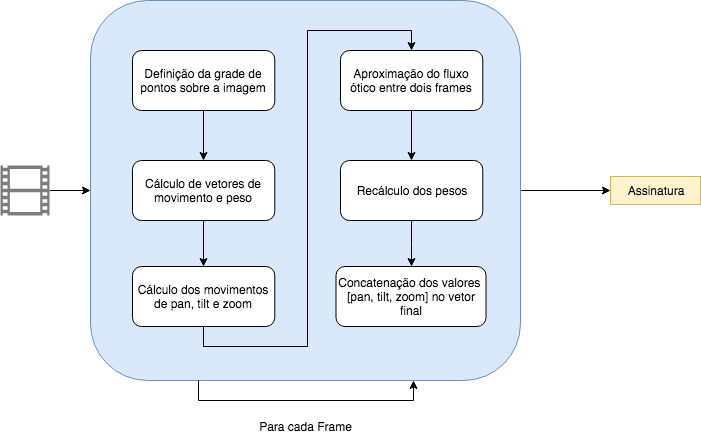
\includegraphics[width=\textwidth]{dados/figuras/diagramas/Diag-CameraMotion}
	\fonte{Autoria própria.}
	\label{fig:dia_cameramotion}
\end{figure}







